

Up until this chapter most of the experiments are done in 1Gbps network environments.
The proposed load balancers have shown decent performance levels in 1Gbps environment.
However, it is essential to investigate the feasibility of the proposed load balancers in 10Gbps network environments.
In this chapter, the author carries out throughput measurements of ipvs-nat, ipvs-tun, and iptables DNAT in 10Gbps environment.
Then the author improves the performance levels of ipvs-nat and ipvs-tun by setting up these load balancers in the node net namespace.
Also presented is the novel software load balancer using eXpress Data Plane(XDP) technology, as an alternative to ipvs software load balancers.

\section{Throughput measurement in 10G network}

In order to evaluate performace levels of proposed load balancer, the author carried out throughput measurement in 10Gbps network environment. 
Table~\ref{tab:hw_sw_spec_10g} shows the hardware and software specification used in the experiment.

{
\setlength{\tabcolsep}{1em}
\renewcommand{\arraystretch}{1.2}

\begin{table}[h]
  \centering
  \begin{tabular}{ll}
    \hline 
    \multicolumn{2}{l}{[Hardware Specification]}   \\
    & CPU: Xeon E5-2450 2.10GHz x 8 (with Hyper Threading) \\
    & Memory: 32GB \\
    & NIC: Intel X550 with 64 rx-queues (16 activated), 10 Gbps \\
    & (Node x 6, Load Balancer x 1, Client x 1)) \\
    & \\
    \multicolumn{2}{l}{[Node Software]}  \\
    & OS: Debian 9.5, linux-4.16.8 \\
    & Kubernetes v1.5.2 \\
    & flannel v0.7.0 \\
    & etcd version: 3.0.15 \\
    & \\
    \multicolumn{2}{l}{[Container Software]}   \\
    & Keepalived: v1.3.2 (12/03,2016) \\
    & nginx : 1.15.4(web server) \\
  \hline 
  \end{tabular}
  \par\bigskip
  \centering
  \begin{minipage}{0.9\columnwidth}
    \caption[Hardware and software specifications for 10Gbps experiment]{
      Hardware and software specifications for 10Gbps experiment.
      There are 16 rx queues activated for the NIC, to match the number of logical CPUs.
    }
    \label{tab:hw_sw_spec_10g}
  \end{minipage}
\end{table}
}

Figure~\ref{fig:ipvs_l3dsr_10g} shows the throughput of ipvs-tun, ipvs-nat and iptables DNAT in 10Gbps environment.
We can see the general characteristics of a load balancer where the throughput increases linearly to a certain level as the number of nginx container increases, and then eventually saturates.
These saturation levels are the performance limits of each of the load balancers, which is determined by packet forwarding efficiency or the bandwidth of the network.
The performance limit of the iptables DNAT is close to 780k [req/sec], where the CPU usage of the benchmark client becomes 100\%.
The performance levels of ipvs and ipvs-tun are inferior to that of iptables DNAT. 

\begin{figure}[h]
  \centering
  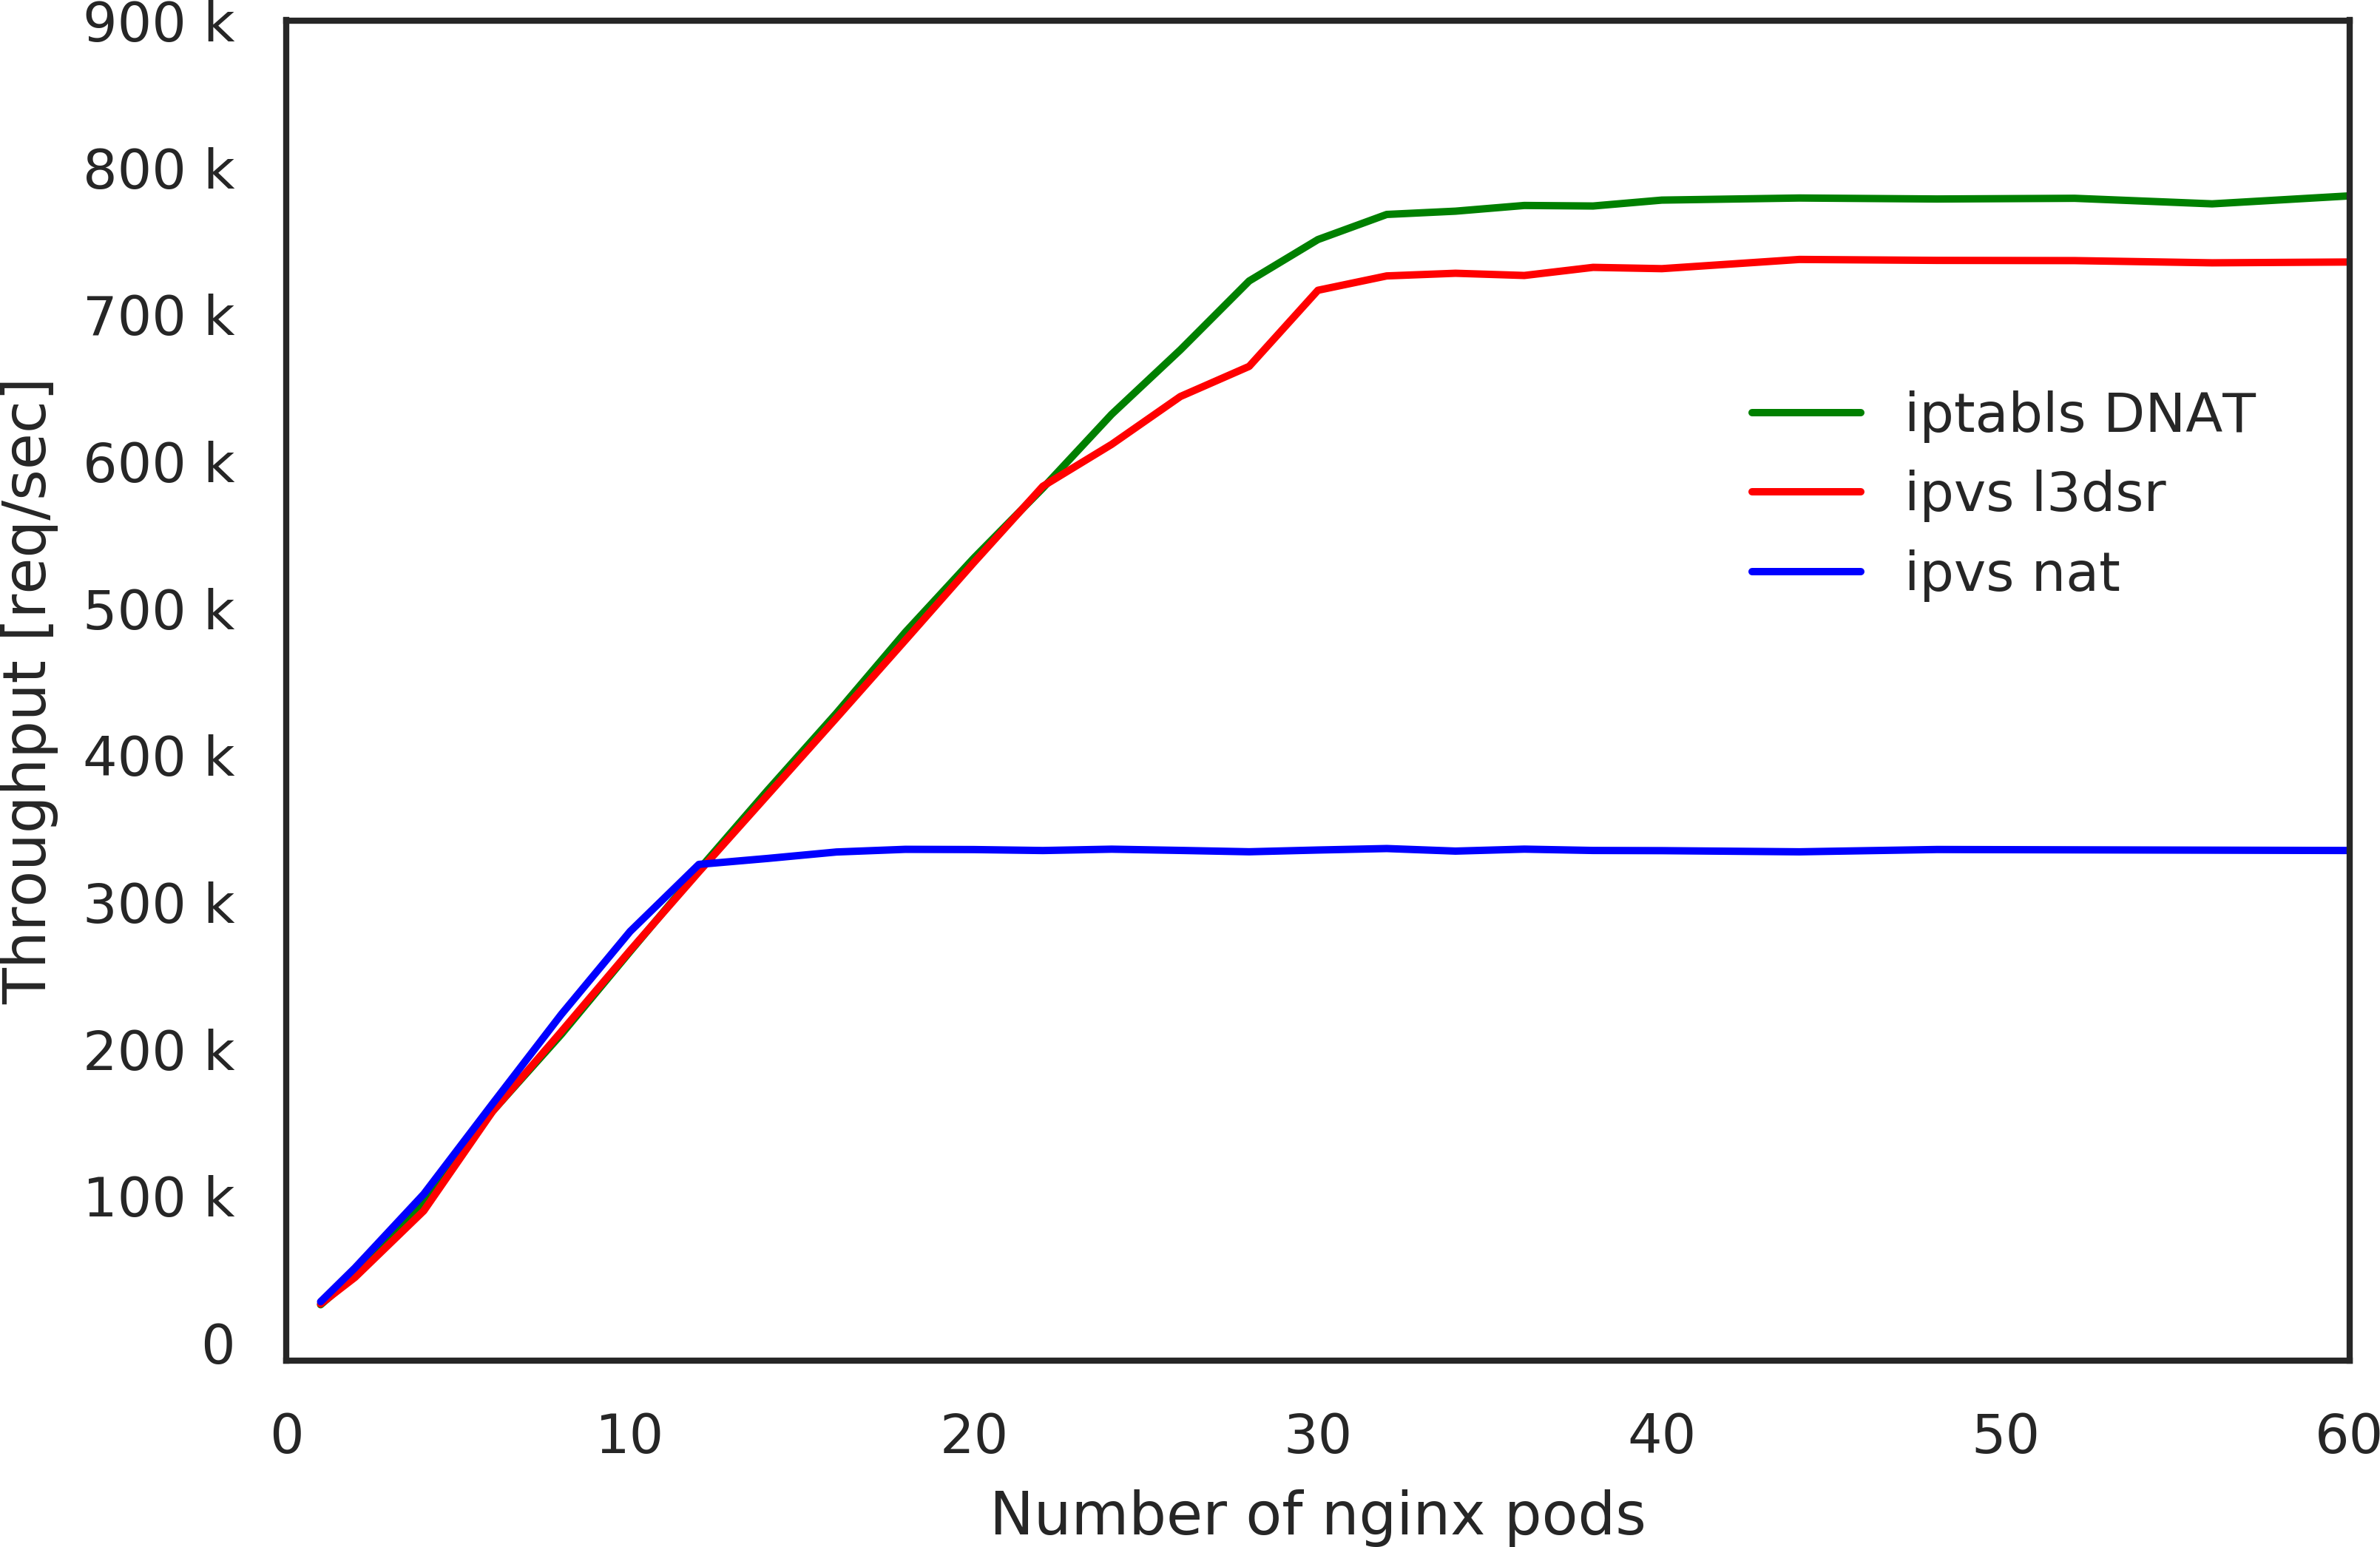
\includegraphics[width=0.8\columnwidth]{Figs/ipvs_l3dsr_10g}
  \par\bigskip
  \centering
  \begin{minipage}{0.9\columnwidth}
    \caption[Throughput of load balancers in 10 Gbps]{
      Throughput of load balancers in 10 Gbps.
      The iptables DNAT rules on the node act as internal load balancer for Kubernetes.
      The ipvs and ipvs-tun are in containers.
      The throughput of the iptables DNAT rules is highest.
    }
    \label{fig:ipvs_l3dsr_10g}
  \end{minipage}
\end{figure}

Figure~\ref{fig:ipvs_node_l3dsr_10g} shows the throughput of ipvs and ipvs-tun in the node namespace together with the throughput of the iptables DNAT.
The throughput of the ipvs and ipvs-tun are improved from the case of the ipvs in container netnamespace.
The throughput of the ipvs-tun is almost identical to that of iptables DNAT, which is limited by CPU power of the benchmark client. 
%
%Although the throughput of the ipvs-nat is smaller than that of the iptables DNAT, it is clearly improved from the result in Figure~\ref{fig:ipvs_l3dsr_10g}.

\begin{figure}[h]
  \centering
  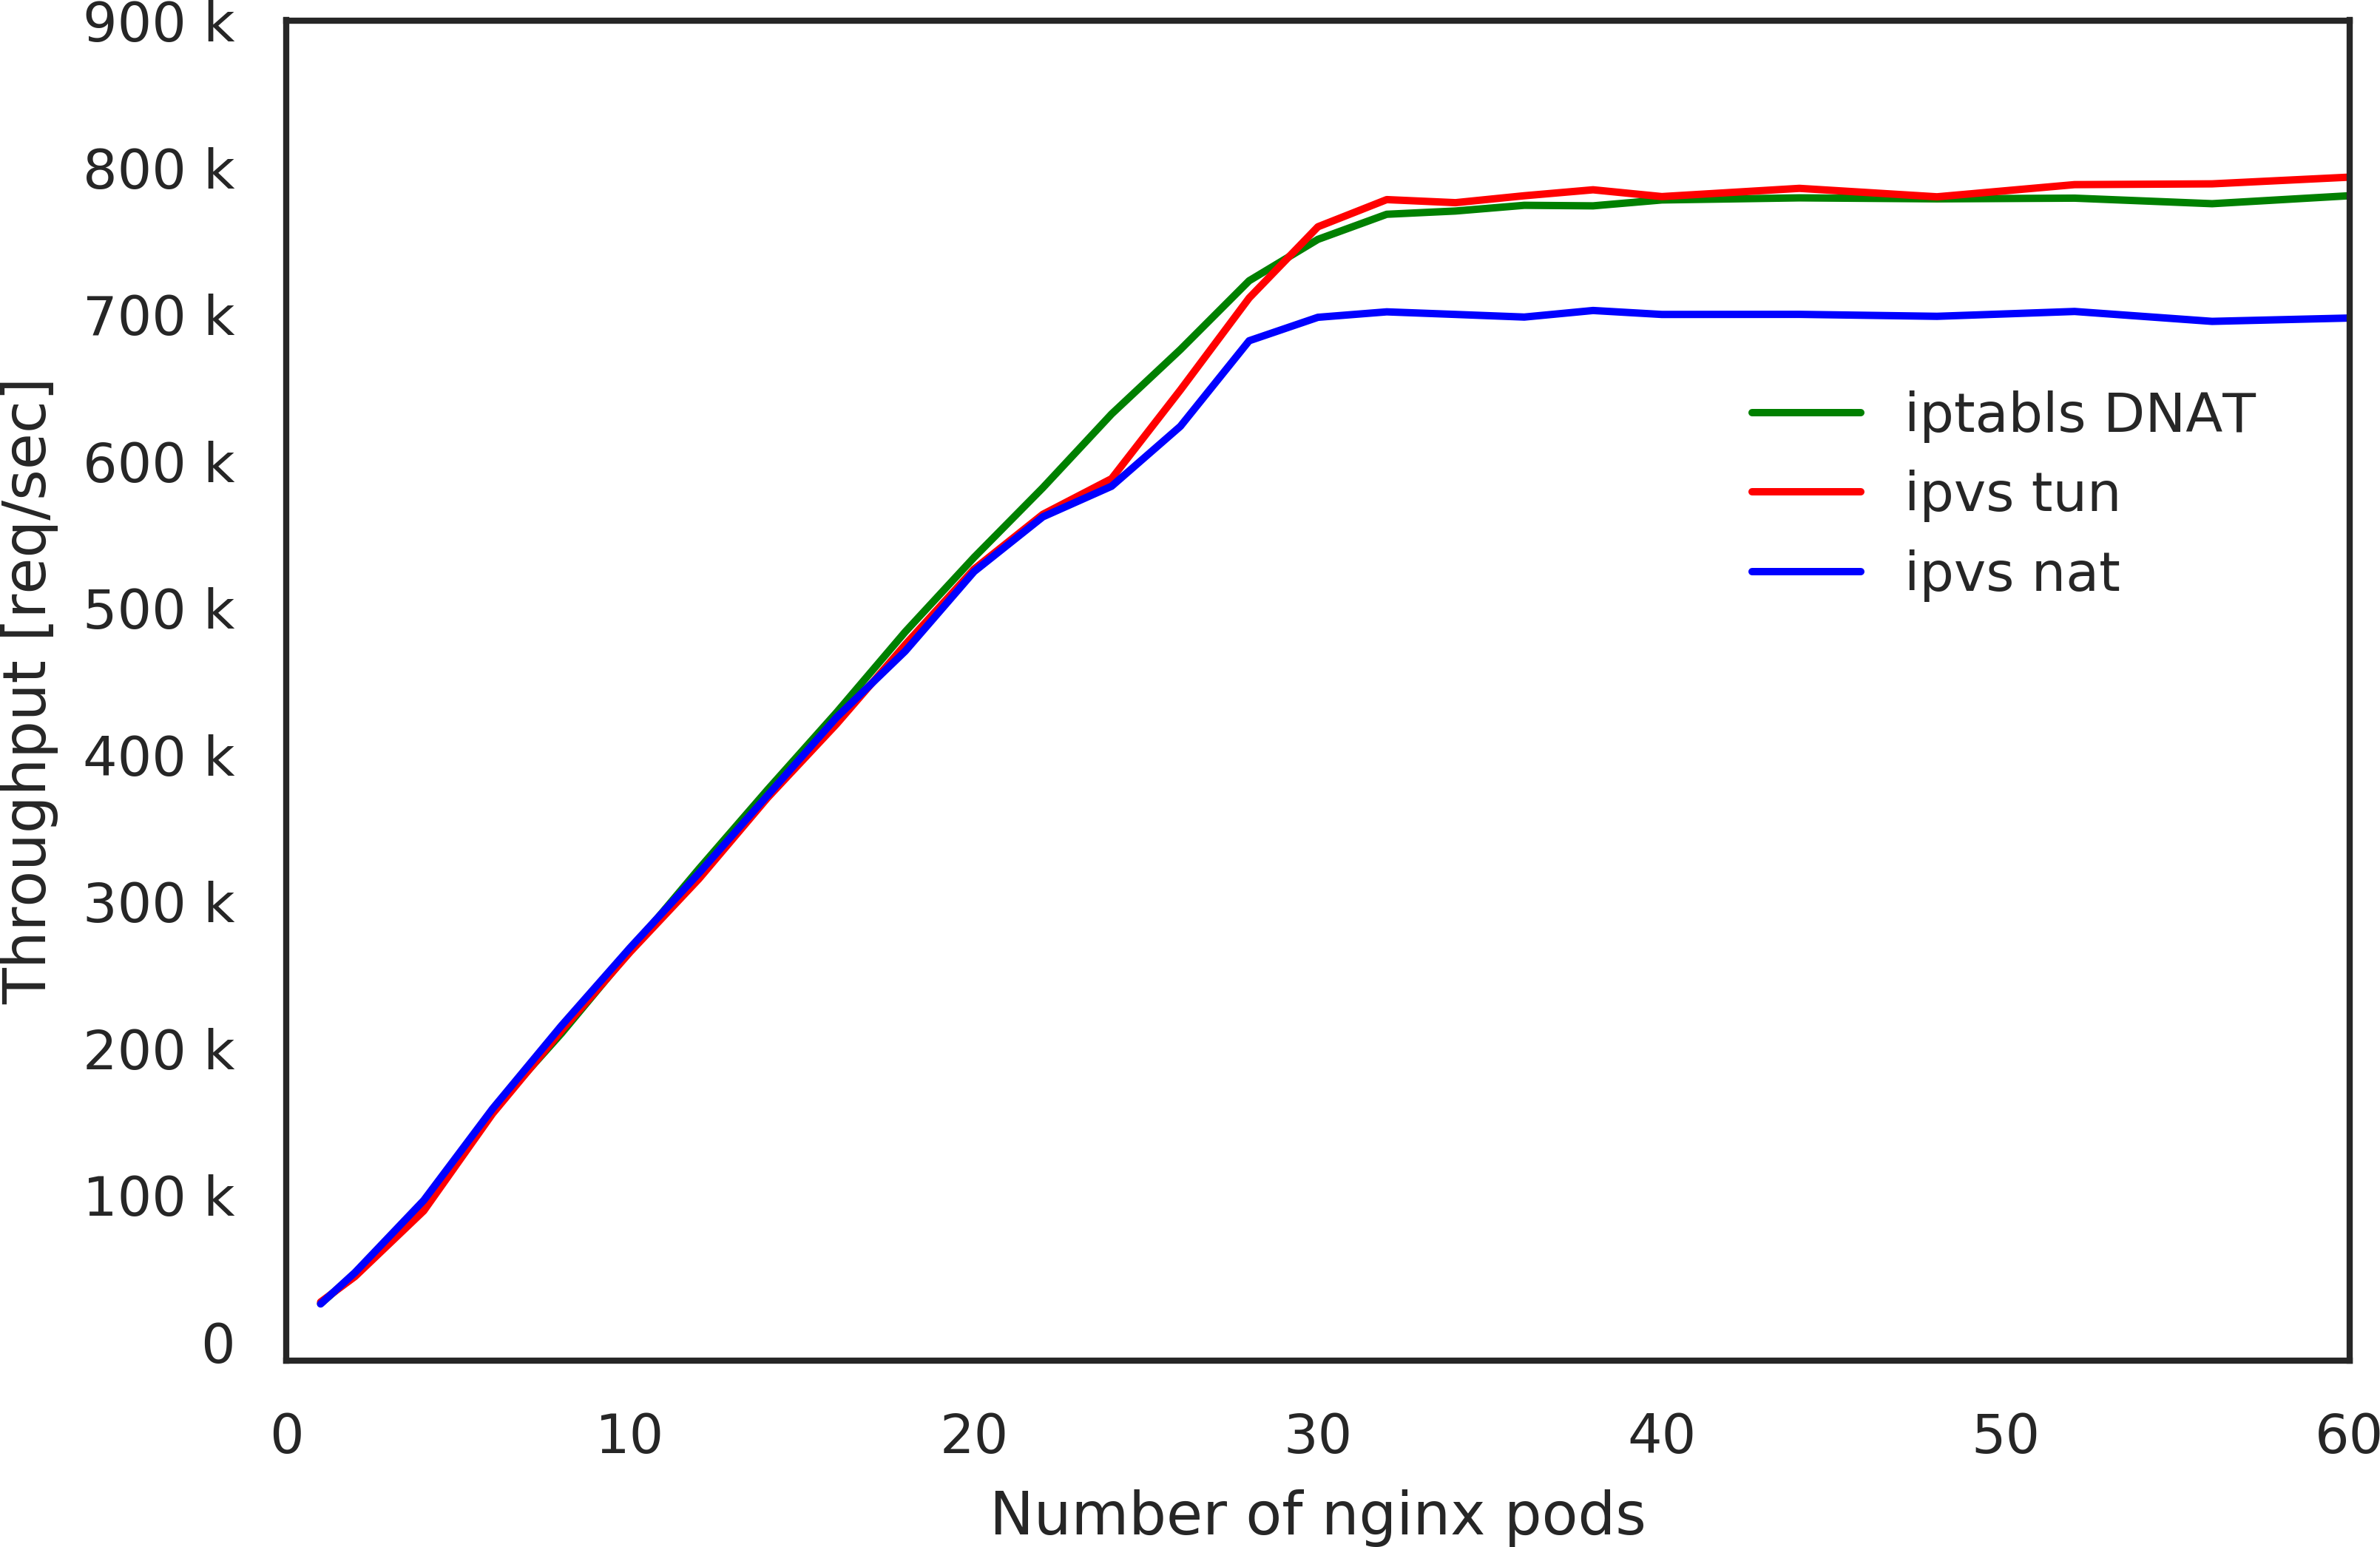
\includegraphics[width=0.8\columnwidth]{Figs/ipvs_node_l3dsr_10g}
  \par\bigskip
  \centering
  \begin{minipage}{0.9\columnwidth}
    \caption[Throughput of load balancers in node namespace]{
      Throughput of load balancers in node namespace.
      The performance levels of the ipvs and ipvs-tun are greatly improved those in \ref{fig:ipvs_l3dsr_10g} by placing them in node net namespace.
    }
    \label{fig:ipvs_node_l3dsr_10g}
  \end{minipage}
\end{figure}

\begin{figure}[h]
  \centering
  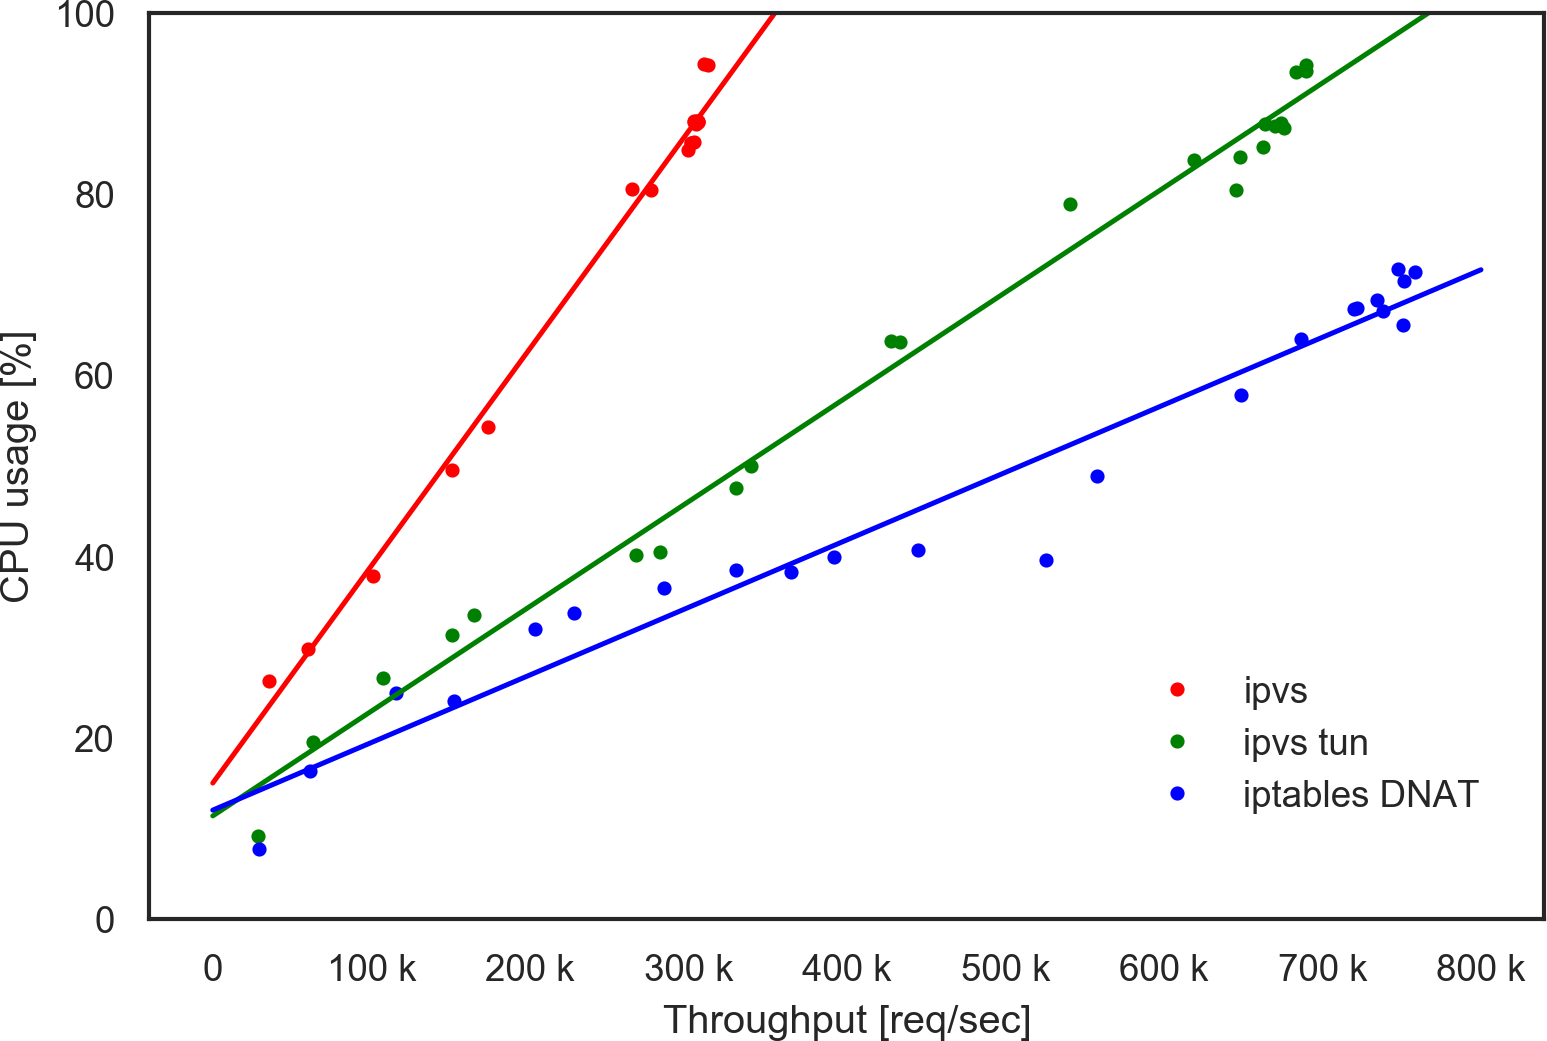
\includegraphics[width=0.8\columnwidth]{Figs/cpu_usage_10g}
  \par\bigskip
  \centering
  \begin{minipage}{0.9\columnwidth}
    \caption[CPU usage of load balancers in containers]{
      CPU usage of load balancers in containers.
      The iptables DNAT rules on the node act as internal load balancer for Kubernetes.
      The ipvs and ipvs-tun are in containers.
      The iptables DNAT consumes the smallest amount of the CPU resource.
    }
    \label{fig:cpu_usage_10g}
  \end{minipage}
\end{figure}

\begin{figure}[h]
  \centering
  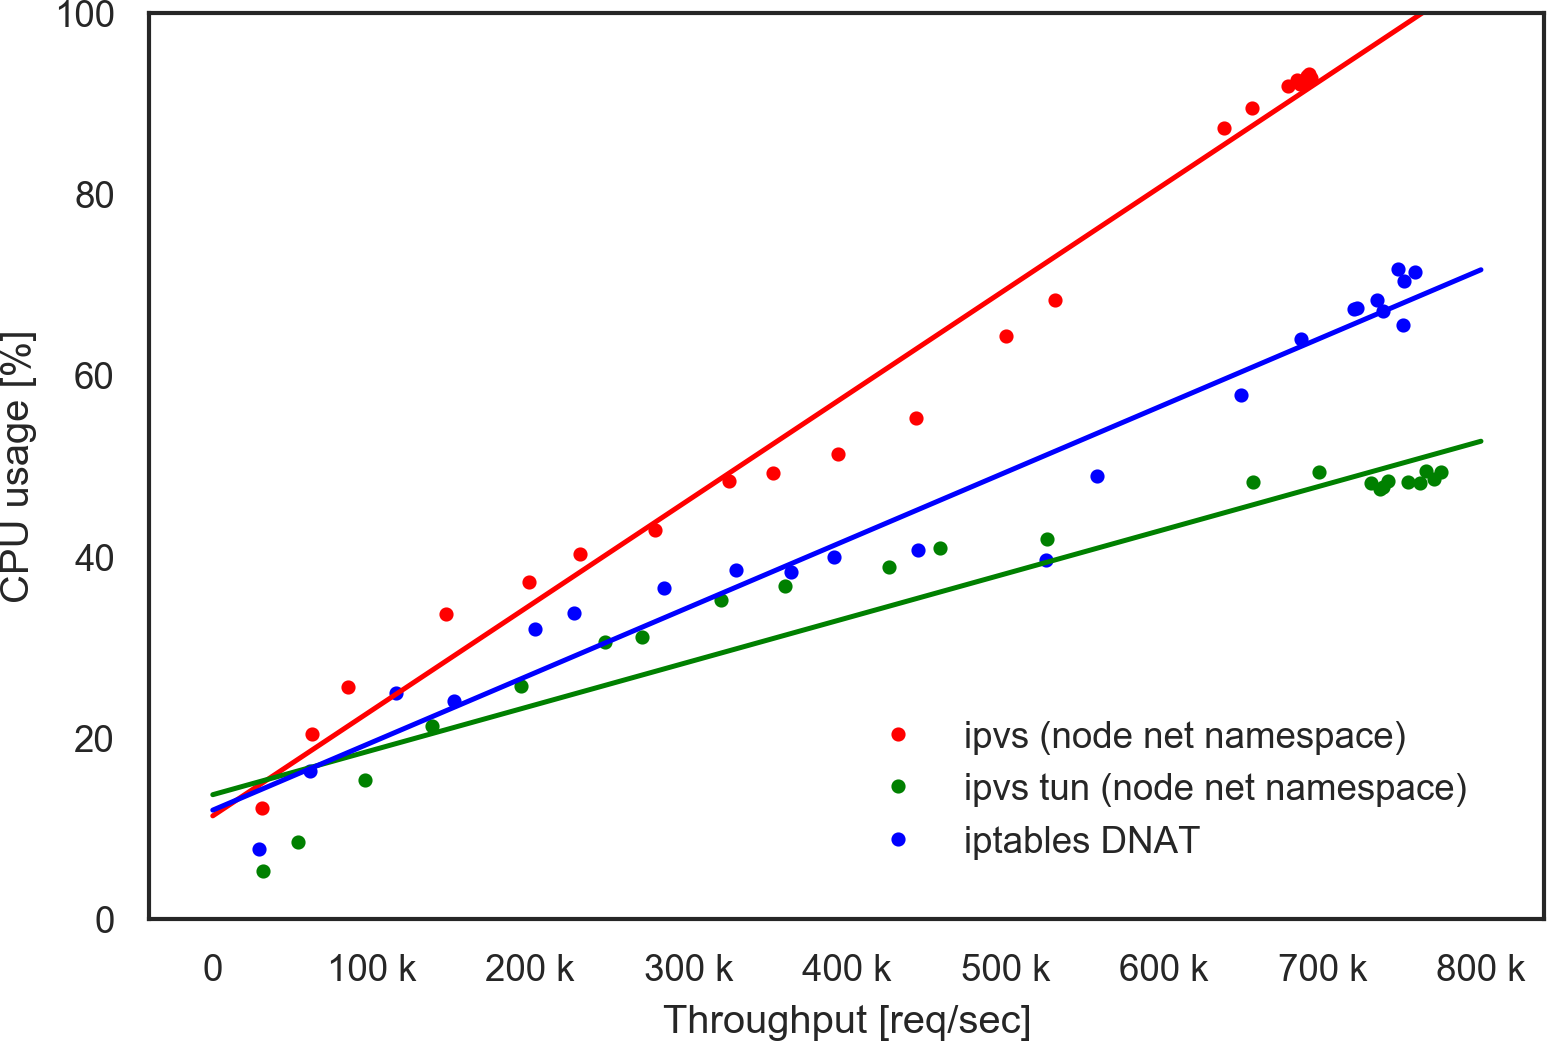
\includegraphics[width=0.8\columnwidth]{Figs/cpu_usage_10g_node_ns}
  \par\bigskip
  \centering
  \begin{minipage}{0.9\columnwidth}
    \caption[CPU usage of load balancers on nodes]{
      CPU usage of load balancers on nodes.
      The iptables DNAT rules on the node act as internal load balancer for Kubernetes.
      The ipvs and ipvs-tun are placed in node netnamespace for comparison. 
      The ipvs-tun consumes the smallest amount of the CPU resource.
    }
    \label{fig:cpu_usage_10g_node_ns}
  \end{minipage}
\end{figure}


\FloatBarrier
\section{XDP load balancer}

[Filled in later]
\mytodo[inline]{Write about XDP}

\begin{figure}[h]
  \centering
  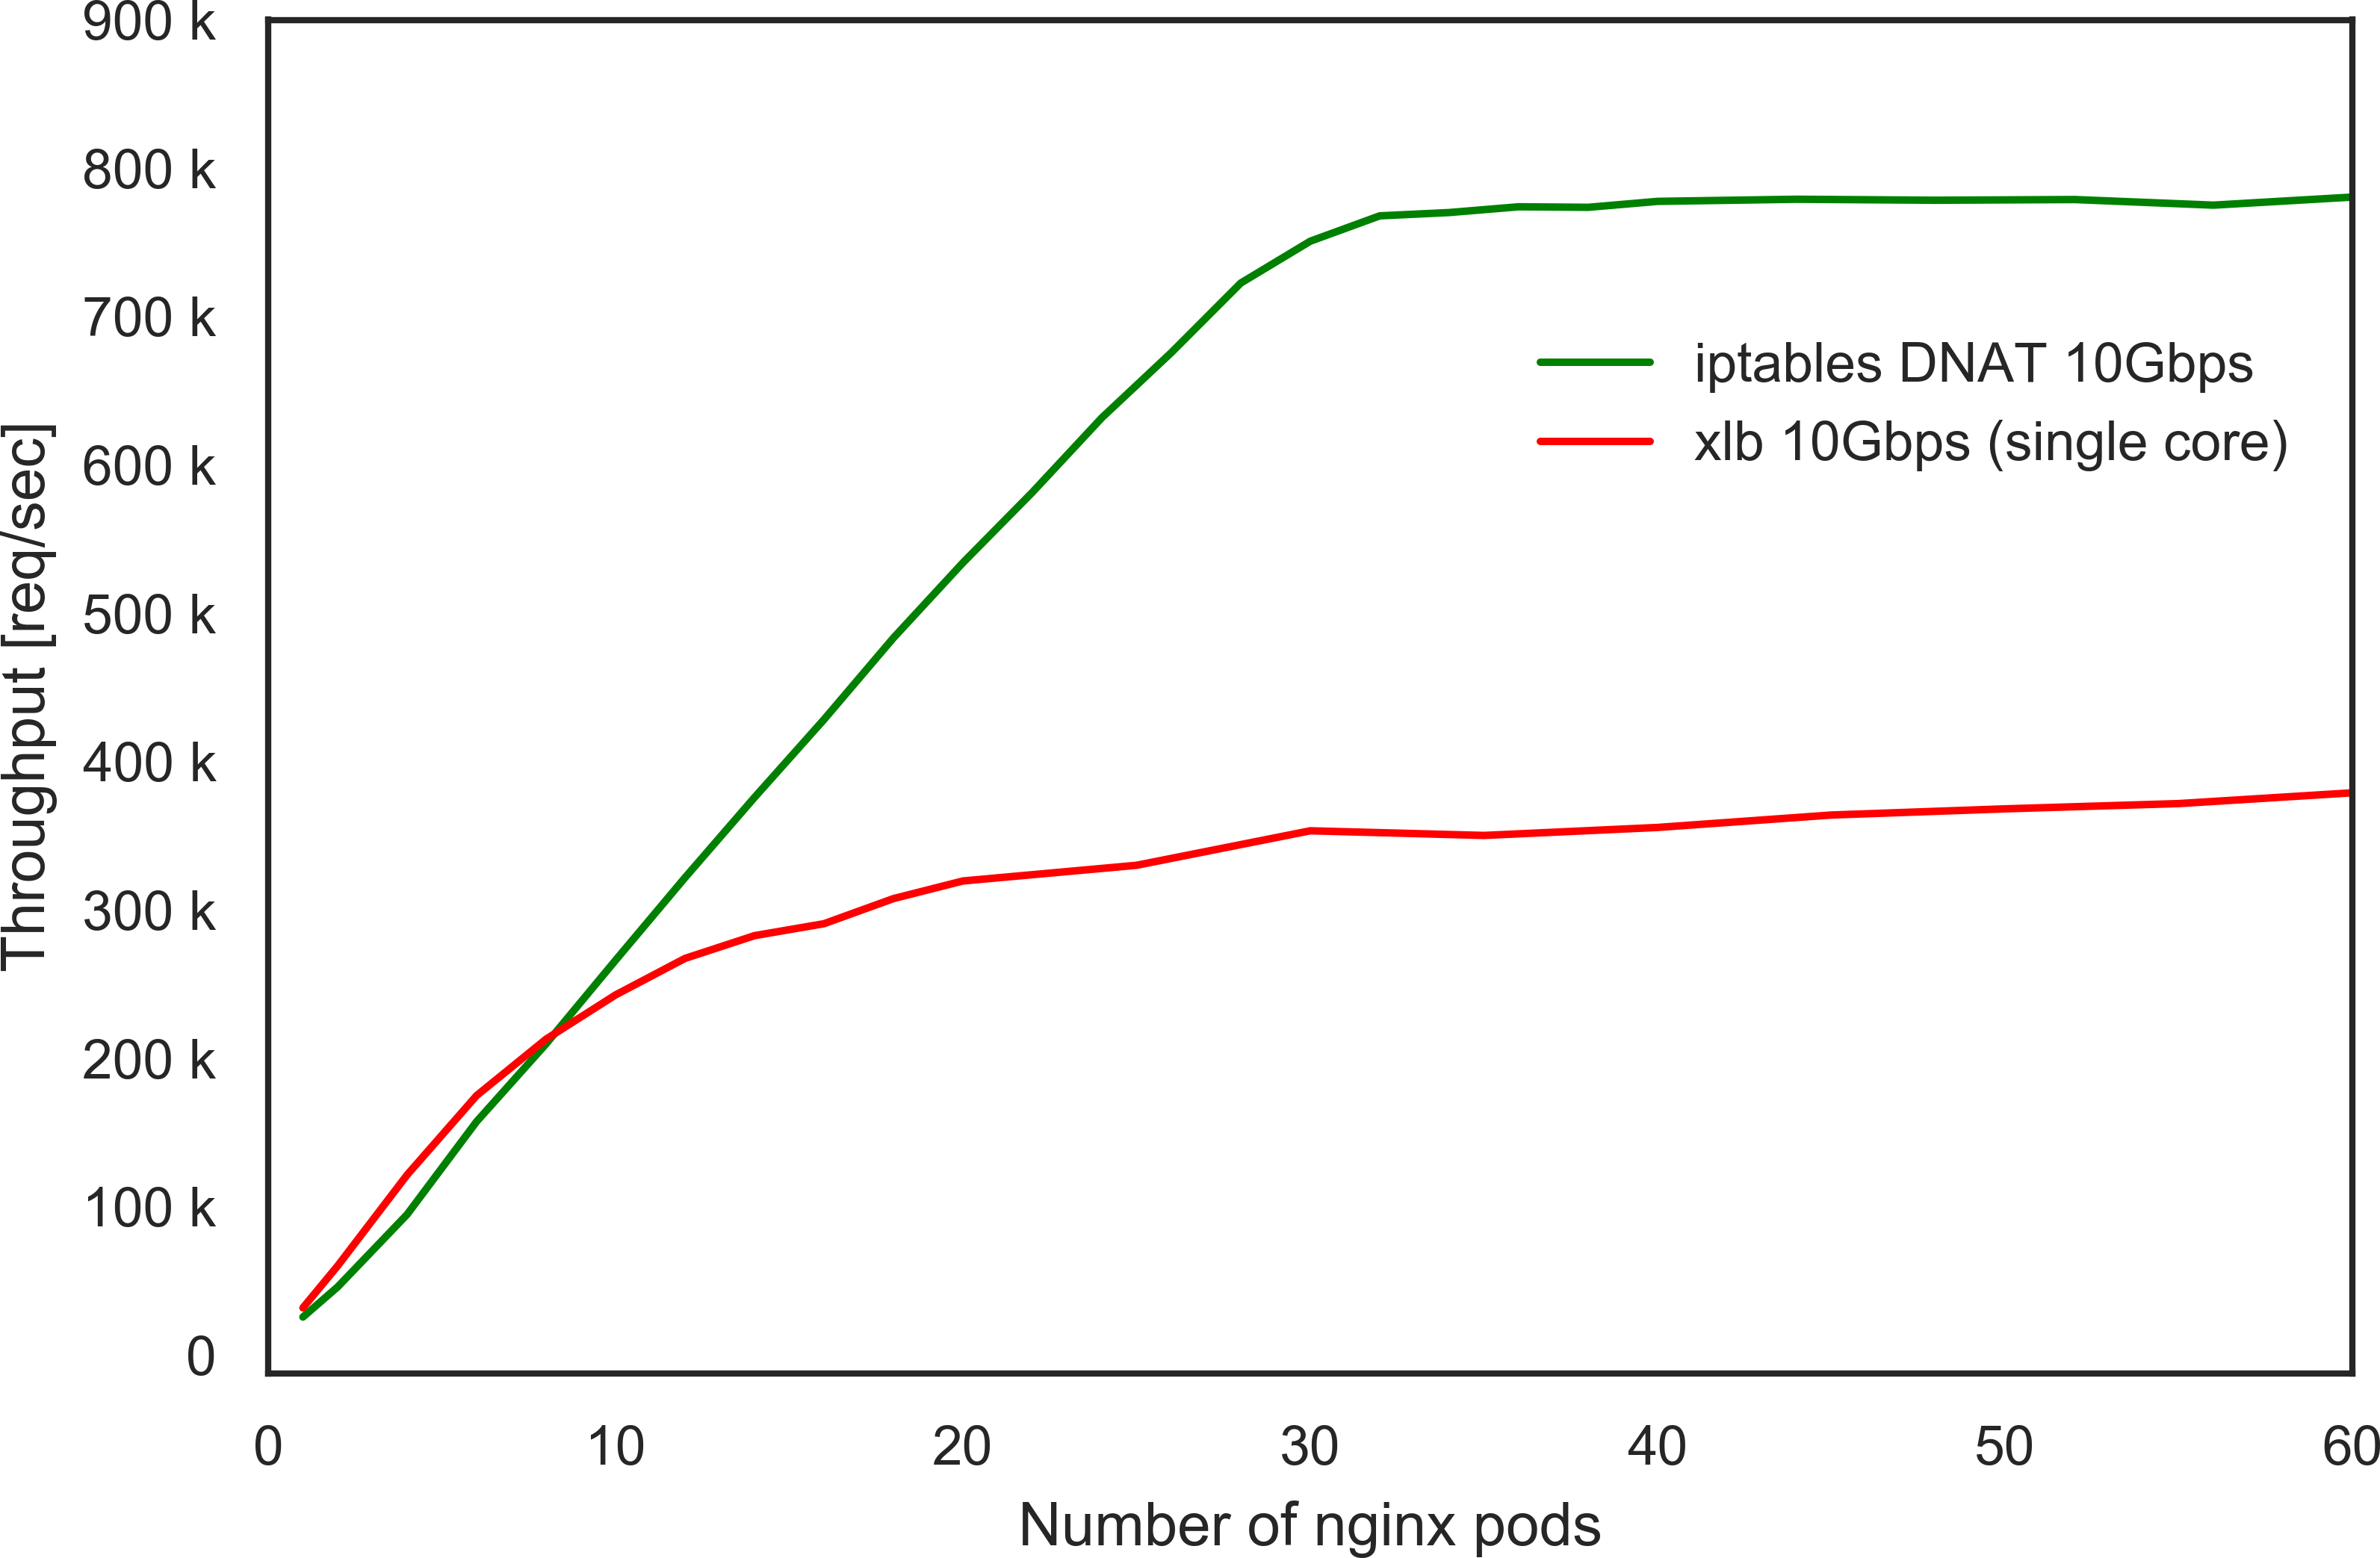
\includegraphics[width=0.8\columnwidth]{Figs/xlb_iptables_dnat_10g}
  \par\bigskip
  \centering
  \begin{minipage}{0.9\columnwidth}
    \caption[Throughput of xlb load balancer]{
      Throughput of xlb load balancer.
      The xlb load balancer is placed in node netnamespace.
      The setting \enquote{(RSS,RPS)=(off,off)}, i.e., single core packet processing is used for the xlb result.
      The setting \enquote{(RSS,RPS)=(on,off)}, i.e., eight core packet processing is used for the iptables DNAT result.
      Although using only a single core, the performance level of the xlb load balancer is close to half of the iptables DNAT's.
    }
    \label{fig:xlb_iptables_dnat_10g}
  \end{minipage}
\end{figure}


\begin{figure}[h]
  \centering
  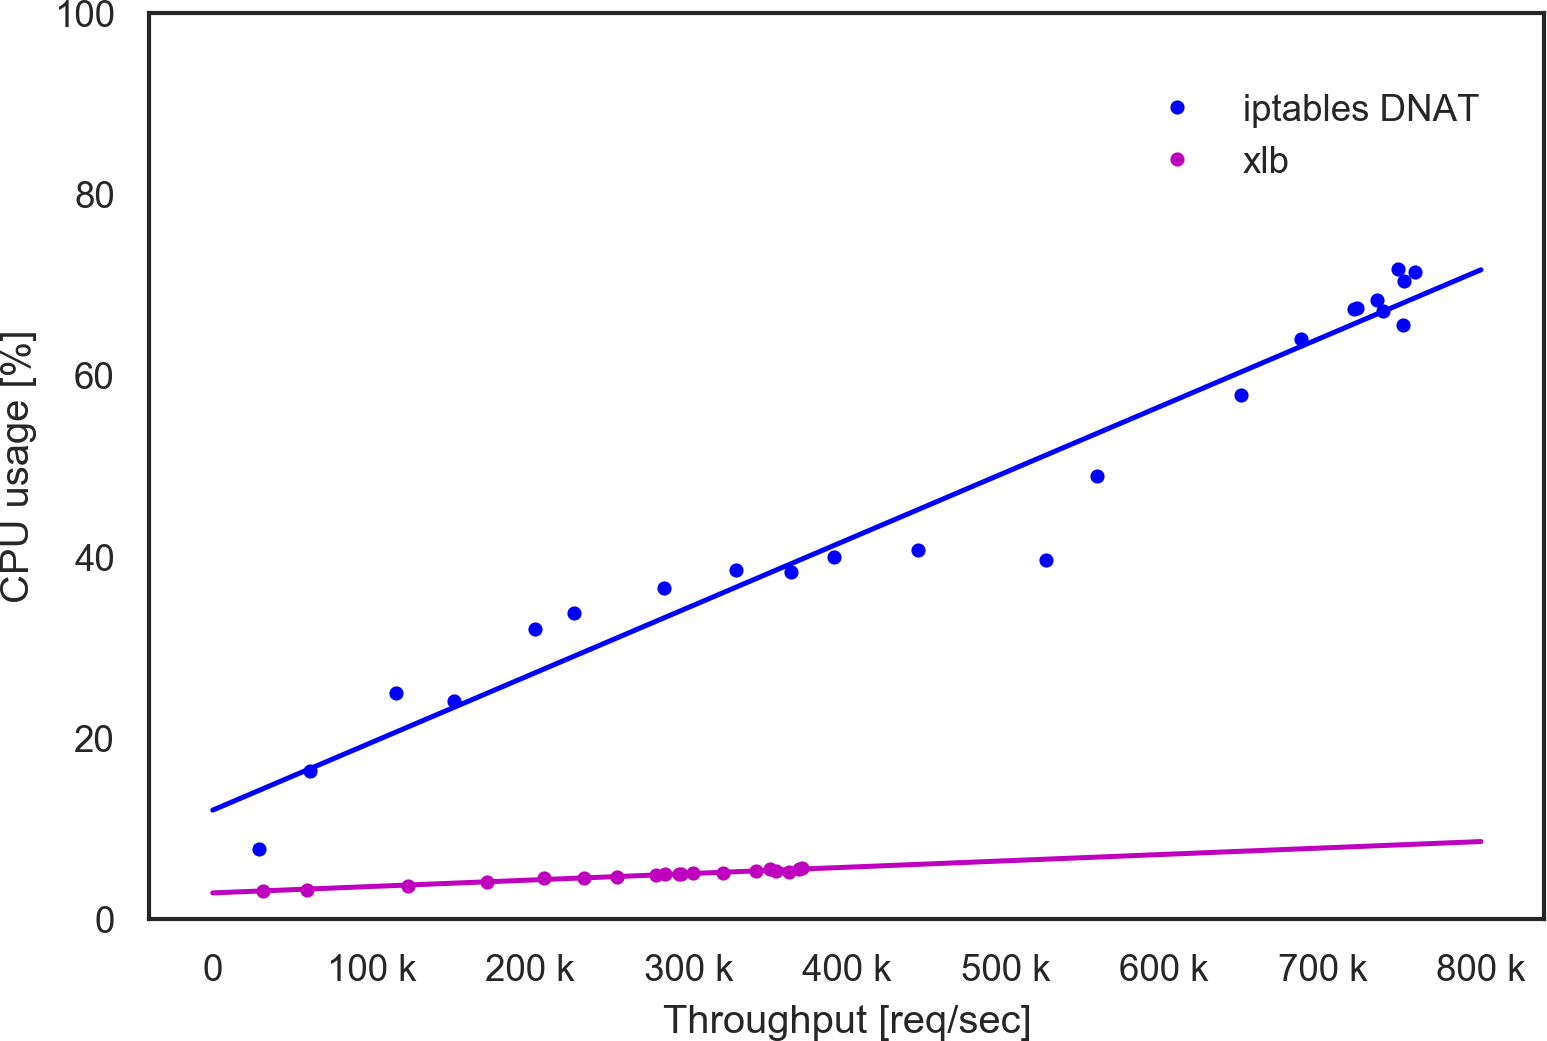
\includegraphics[width=0.8\columnwidth]{Figs/cpu_usage_10g_xlb}
  \par\bigskip
  \centering
  \begin{minipage}{0.9\columnwidth}
    \caption[CPU usage of xlb load balancer]{
      CPU usage of xlb load balancer.
      The xlb uses much less CPU resource than iptables DNAT.
    }
    \label{fig:cpu_usage_10g_xlb}
  \end{minipage}
\end{figure}

\FloatBarrier

\section{Summary}

In this chapter, the author carried out throughput measurements of ipvs-nat, ipvs-tun, and iptables DNAT in 10Gbps environment.
From the results the general characteristics of a load balancer are observesd.
The throughput increases linearly to a certain level as the number of nginx container increases, and then eventually saturates.
The performance levels for of the load balancers are improved by using 10Gbps network.
However, the throughputs of ipvs-nat and ipvs-tun are smaller than that of iptables DNAT.

Then the author improved the performance levels by setting up ipvs-nat and ipvs-tun load balancers in the node net namespace to remove overhead of the container network.
The throughput of the ipvs-tun became almost identical to that of iptables DNAT, and the throughput of the ipvs-nat also improved to the level close to that of the iptables DNAT.

%% The authot also presented the novel software load balancer using eXpress Data Plane(XDP) technology, as an alternative to ipvs software load balancers.
[Filled in later]
\mytodo[inline]{Write summary about XDP}



Load balancer in containers under performed and consumed more CPU resources than iptables DNAT on a node.
Container network that utilize bridge+veth maybe inefficient.
Better network set up for container is needed.

Maximum throughputs of ipvs-tun on a node and iptables DNAT are equivalent in the experiment, which is because the benchmark client can not measure throughput more than 800K [req/sec].
However the ipvs-tun consumed less CPU resouces than iptables DNAT.
Performance level of ipvs on the node is lower than of iptables DNAT.
The ipvs consumed more CPU resources than iptables DNAT.
Better software load balancers are needed.

The xlb load balancer has better per core throughput than iptables DNAT.
The xlb load balancer much less CPU resources than iptables DNAT.
The author plan to improve the perfomance levels of the xlb load balancer by enabling multicore packet processing. 


Band width limitations of 10G are 1.9M req/sec and 2.7M req/sec for ipvs and ipvs-tun, respectively.
Neither ipvs and iptables DNAT does not have that levels of performance. 

